
\documentclass[compress]{beamer}
\usepackage{ifthen,verbatim}

\title{Muon Alignment Status Report}
\author{\underline{Jim~Pivarski}, Alexei~Safonov, Karoly~Banicz$^*$, Vadim~Khotilovich, Alexey~Kamenev$^{**}$}
\institute{Texas A\&M University \\ $^*$Purdue University \\ $^{**}$Joint Institute for Nuclear Research, Dubna}
\date{20 October, 2007}

\newcommand{\isnote}{}
\xdefinecolor{lightyellow}{rgb}{1.,1.,0.25}
\xdefinecolor{darkblue}{rgb}{0.1,0.1,0.7}

%% Uncomment this to get annotations
%% \def\notes{\addtocounter{page}{-1}
%%            \renewcommand{\isnote}{*}
%% 	   \beamertemplateshadingbackground{lightyellow}{white}
%%            \begin{frame}
%%            \frametitle{Notes for the previous page (page \insertpagenumber)}
%%            \itemize}
%% \def\endnotes{\enditemize
%% 	      \end{frame}
%%               \beamertemplateshadingbackground{white}{white}
%%               \renewcommand{\isnote}{}}

%% Uncomment this to not get annotations
\def\notes{\comment}
\def\endnotes{\endcomment}

\setbeamertemplate{navigation symbols}{}
\setbeamertemplate{headline}{\includegraphics[height=1 cm]{../cmslogo} \hspace{0.1 cm} \includegraphics[height=1 cm]{../tamulogo} \hfill
\begin{minipage}{5.5 cm}
\vspace{-0.75 cm} \small
\begin{center}
\ifthenelse{\equal{\insertpagenumber}{1}}{}{\textcolor{blue}{\insertsection}}
\end{center}
\end{minipage} \hfill
\begin{minipage}{4.5 cm}
\vspace{-0.75 cm} \small
\begin{flushright}
\ifthenelse{\equal{\insertpagenumber}{1}}{}{Jim Pivarski \hspace{0.5 cm} \insertpagenumber\isnote/\pageref{numpages}}
\end{flushright}
\end{minipage}\mbox{\hspace{0.2 cm}}}

\begin{document}
\frame{\titlepage}

%% \begin{notes}
%% \item This is the annotated version of my talk.
%% \item If you want the version that I am presenting, download the one
%% labeled ``slides'' on Indico (or just ignore these yellow pages).
%% \item The annotated version is provided for extra detail and a written
%% record of comments that I intend to make orally.
%% \item Yellow notes refer to the content on the {\it previous} page.
%% \item All other slides are identical for the two versions.
%% \end{notes}

\begin{frame}
\frametitle{Main Theme}

The muon alignment {\it process} is basically working (most stations) and
performs better than expected.

\vspace{0.5 cm}
Now we need to
\begin{enumerate}[\hspace{0.5 cm}(\alph{enumi}) ]\setlength{\itemsep}{0.2 cm}
\item continue looking for sources of systematic error
\item correct a bug in ME1/1
\item improve our layer-alignment strategy
\item develop cosmic-ray and beam-halo procedures
\item create additional monitoring tools

\vspace{0.35 cm}

\item {\it actually} align the detector: MTCC as soon as possible, beam-halo and $Z\to\mu\mu$ when available
\end{enumerate}
\end{frame}

\section*{What works}

\begin{frame}
\begin{center}
\Huge \textcolor{blue}{\sc Part I: What Works}
\end{center}
\end{frame}

\begin{frame}
\frametitle{Working procedure}
\begin{columns}
\column{0.4\linewidth}
\mbox{ } \\
Reaches alignment goals with 5~pb$^{-1}$ of $Z$, $W$ (20,000 high-$|\vec{p}|$ muons), assuming no surprises
\column{0.7\linewidth}
\vspace{-0.75 cm} 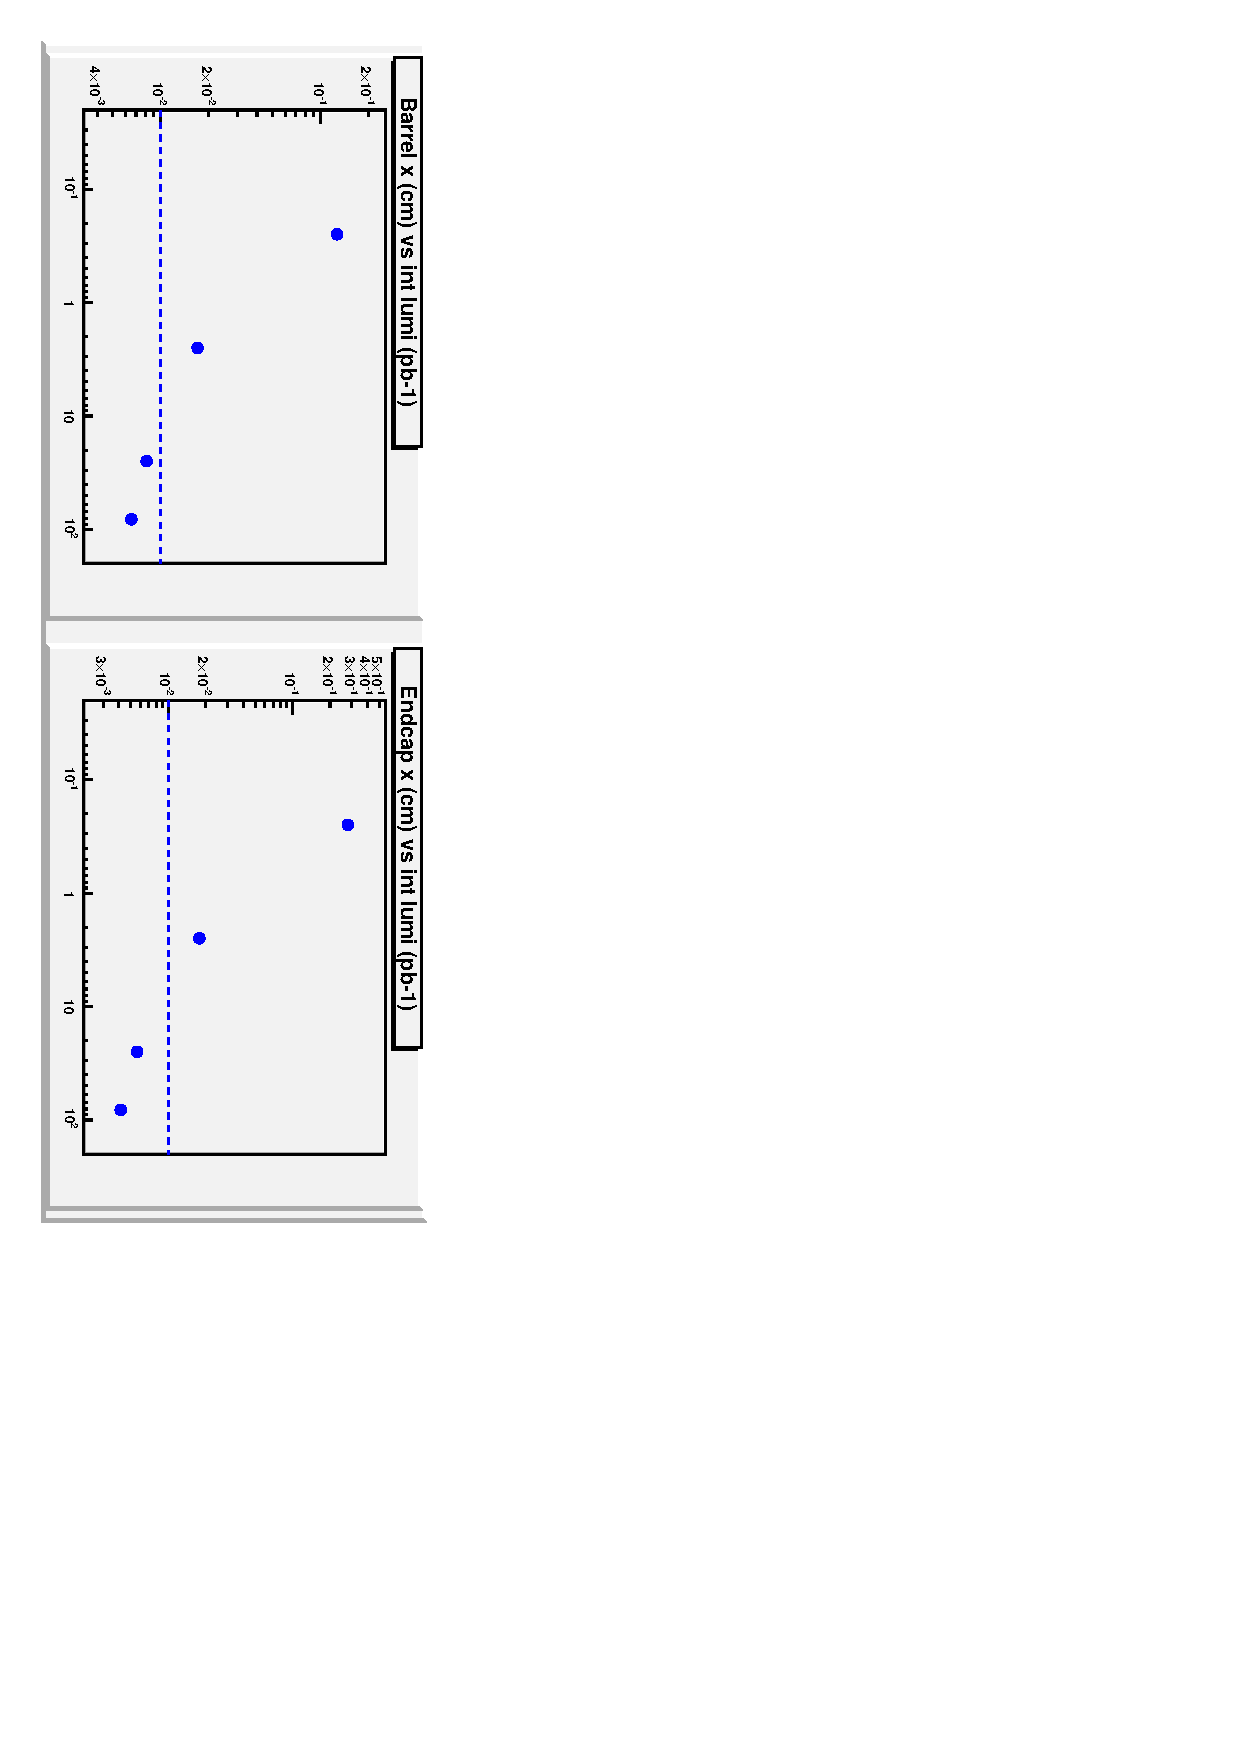
\includegraphics[height=\linewidth, angle=90]{events_x_wacky.pdf}
\end{columns}
\begin{center}
\begin{minipage}{0.8\linewidth}
\begin{columns}
\column{0.5\linewidth}
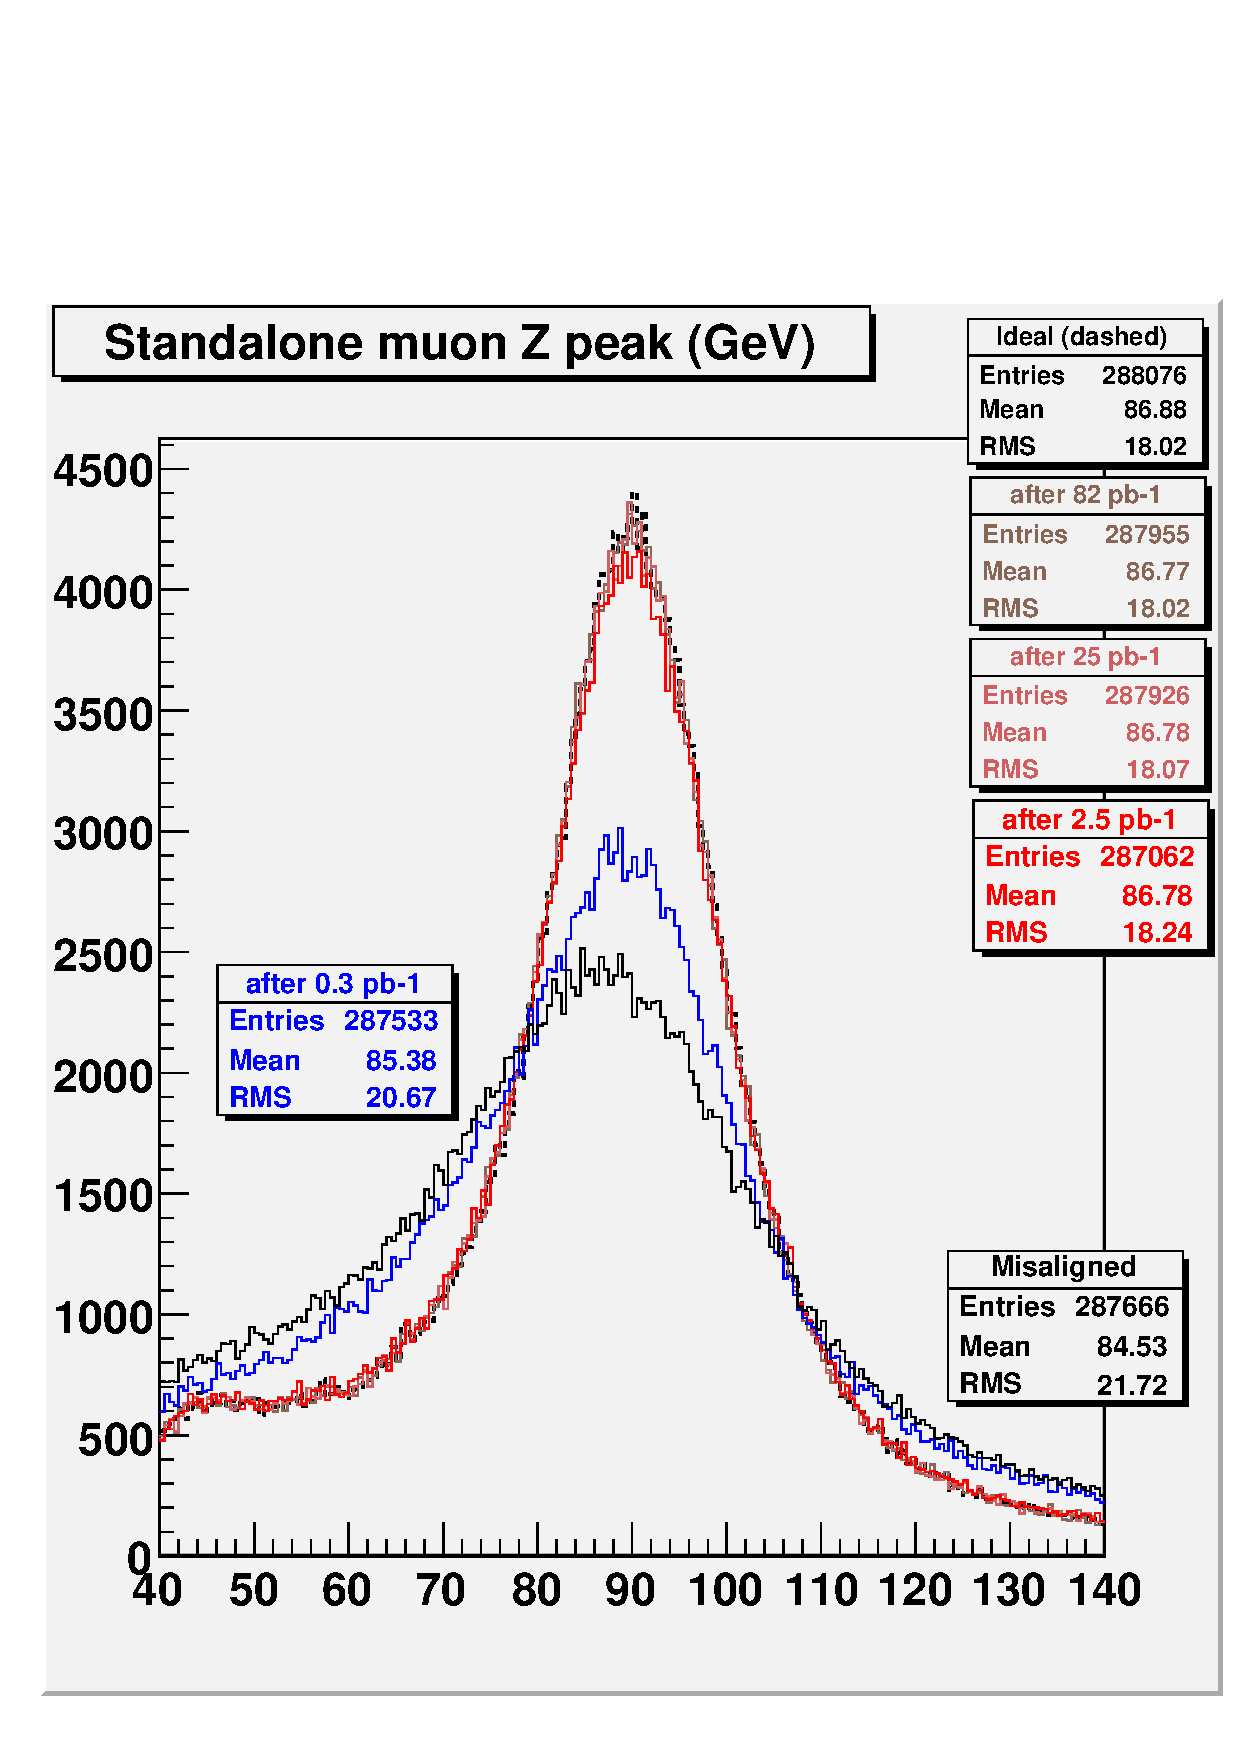
\includegraphics[width=\linewidth]{checkit_standaloneZ.pdf}
\column{0.5\linewidth}
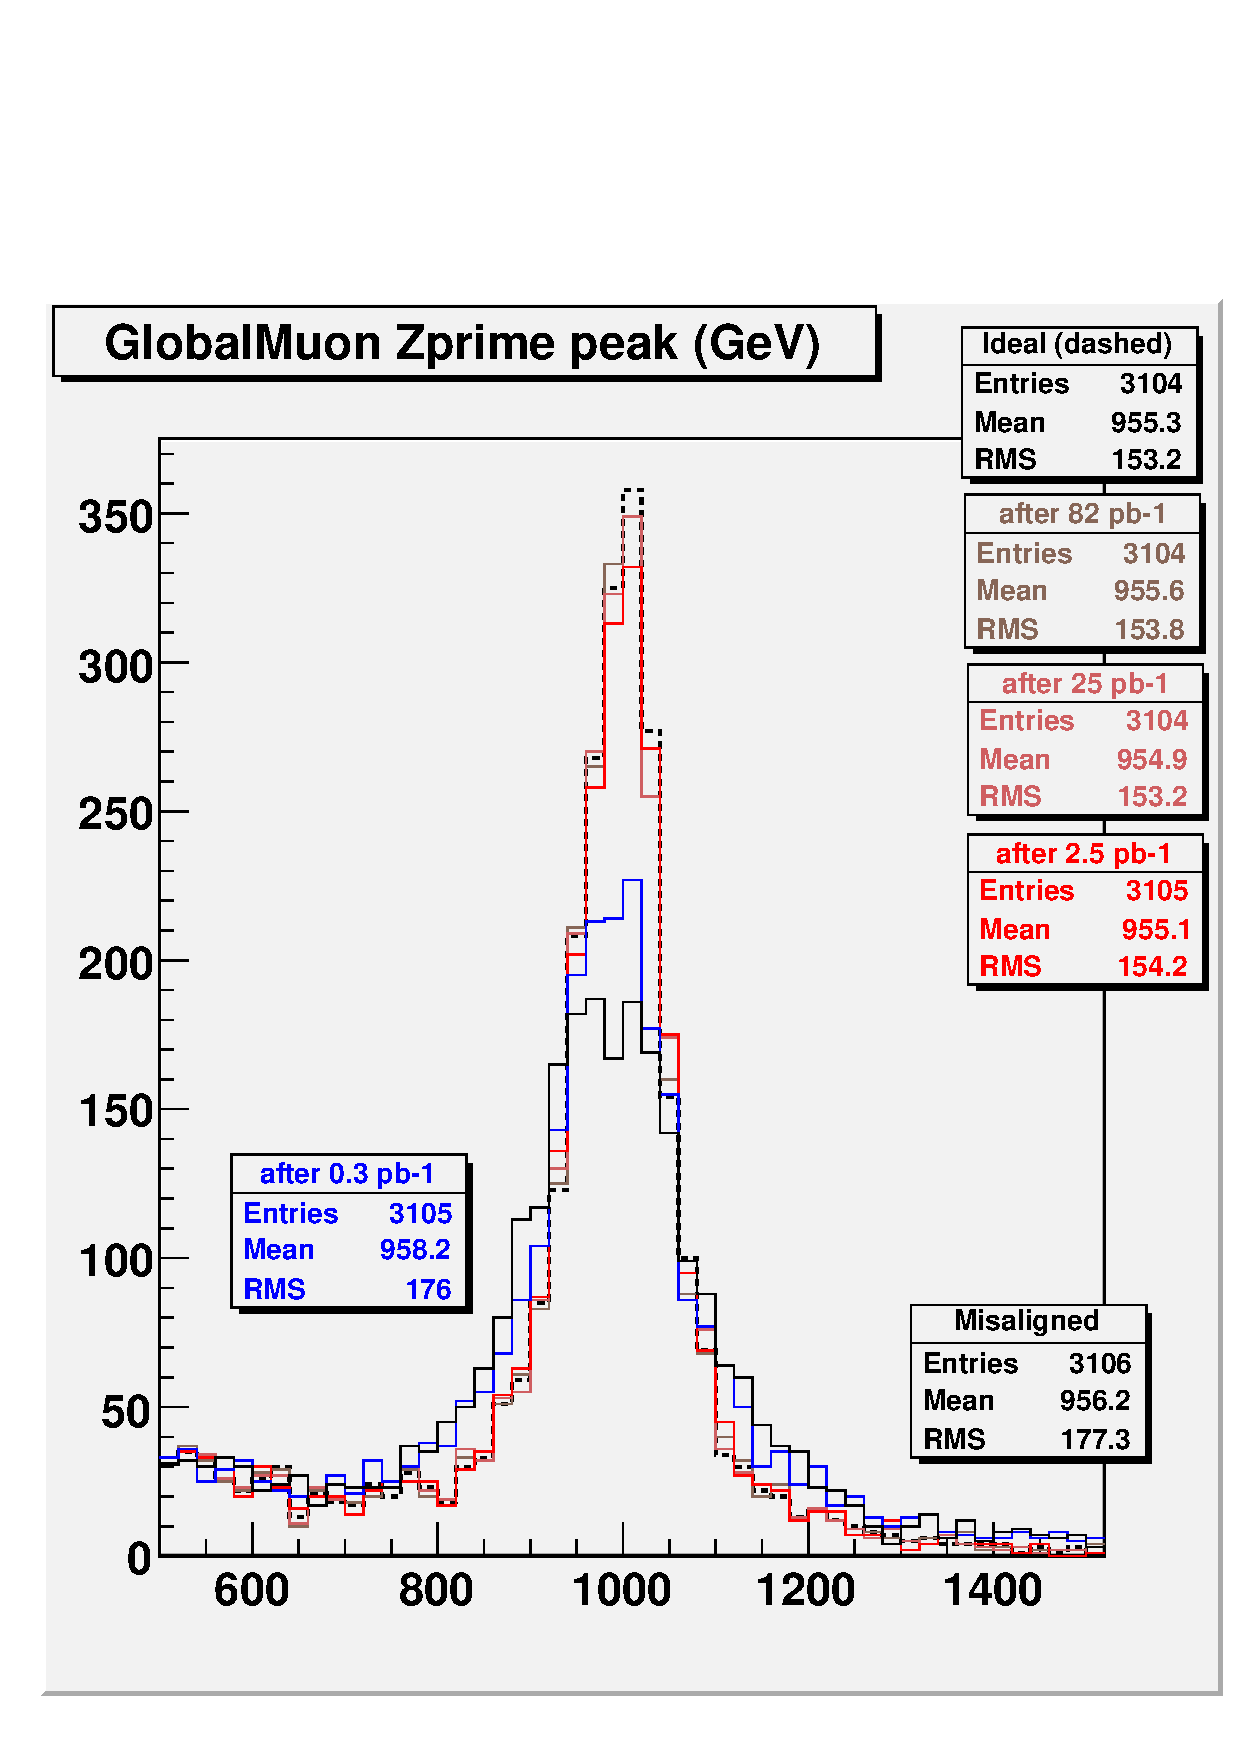
\includegraphics[width=\linewidth]{checkit_globZprime.pdf}
\end{columns}
\end{minipage}
\end{center}
\end{frame}

\begin{frame}
\frametitle{Anticipating surprises: systematics studies}

\vfill
{\large \textcolor{darkblue}{Done}}
\begin{itemize}
\item Dependence on miscalibration: negligible

\item Dependence on tracker misalignment: only significant at 1--2
times the ``tracker short-term scenario''
\end{itemize}

\vfill
{\large \textcolor{darkblue}{Partial}}
\begin{itemize}
\item Dependence on momentum: aligned high-$|\vec{p}|$ $Z\to\mu\mu$
(60$+$~GeV) and low-$|\vec{p}|$ $Z\to\mu\mu$ ($\sim$20 to 60~GeV), but not
realistic physics distributions

\vspace{0.2 cm}
low-$|\vec{p}|$: 10\% of chambers placed at too large radius (2--8~mm)
\end{itemize}

\vfill
{\large \textcolor{darkblue}{To-do}}
\begin{itemize}
\item Mismeasured magnetic field

\item Incorrect material budget/distribution

\item Backgrounds (contamination with non-muons)
\end{itemize}
\end{frame}

\begin{frame}
\frametitle{All systematics studies applied to \only<2>{2 }TeV Drell-Yan and $Z'$}
\begin{columns}
\column{0.5\linewidth}
\only<1>{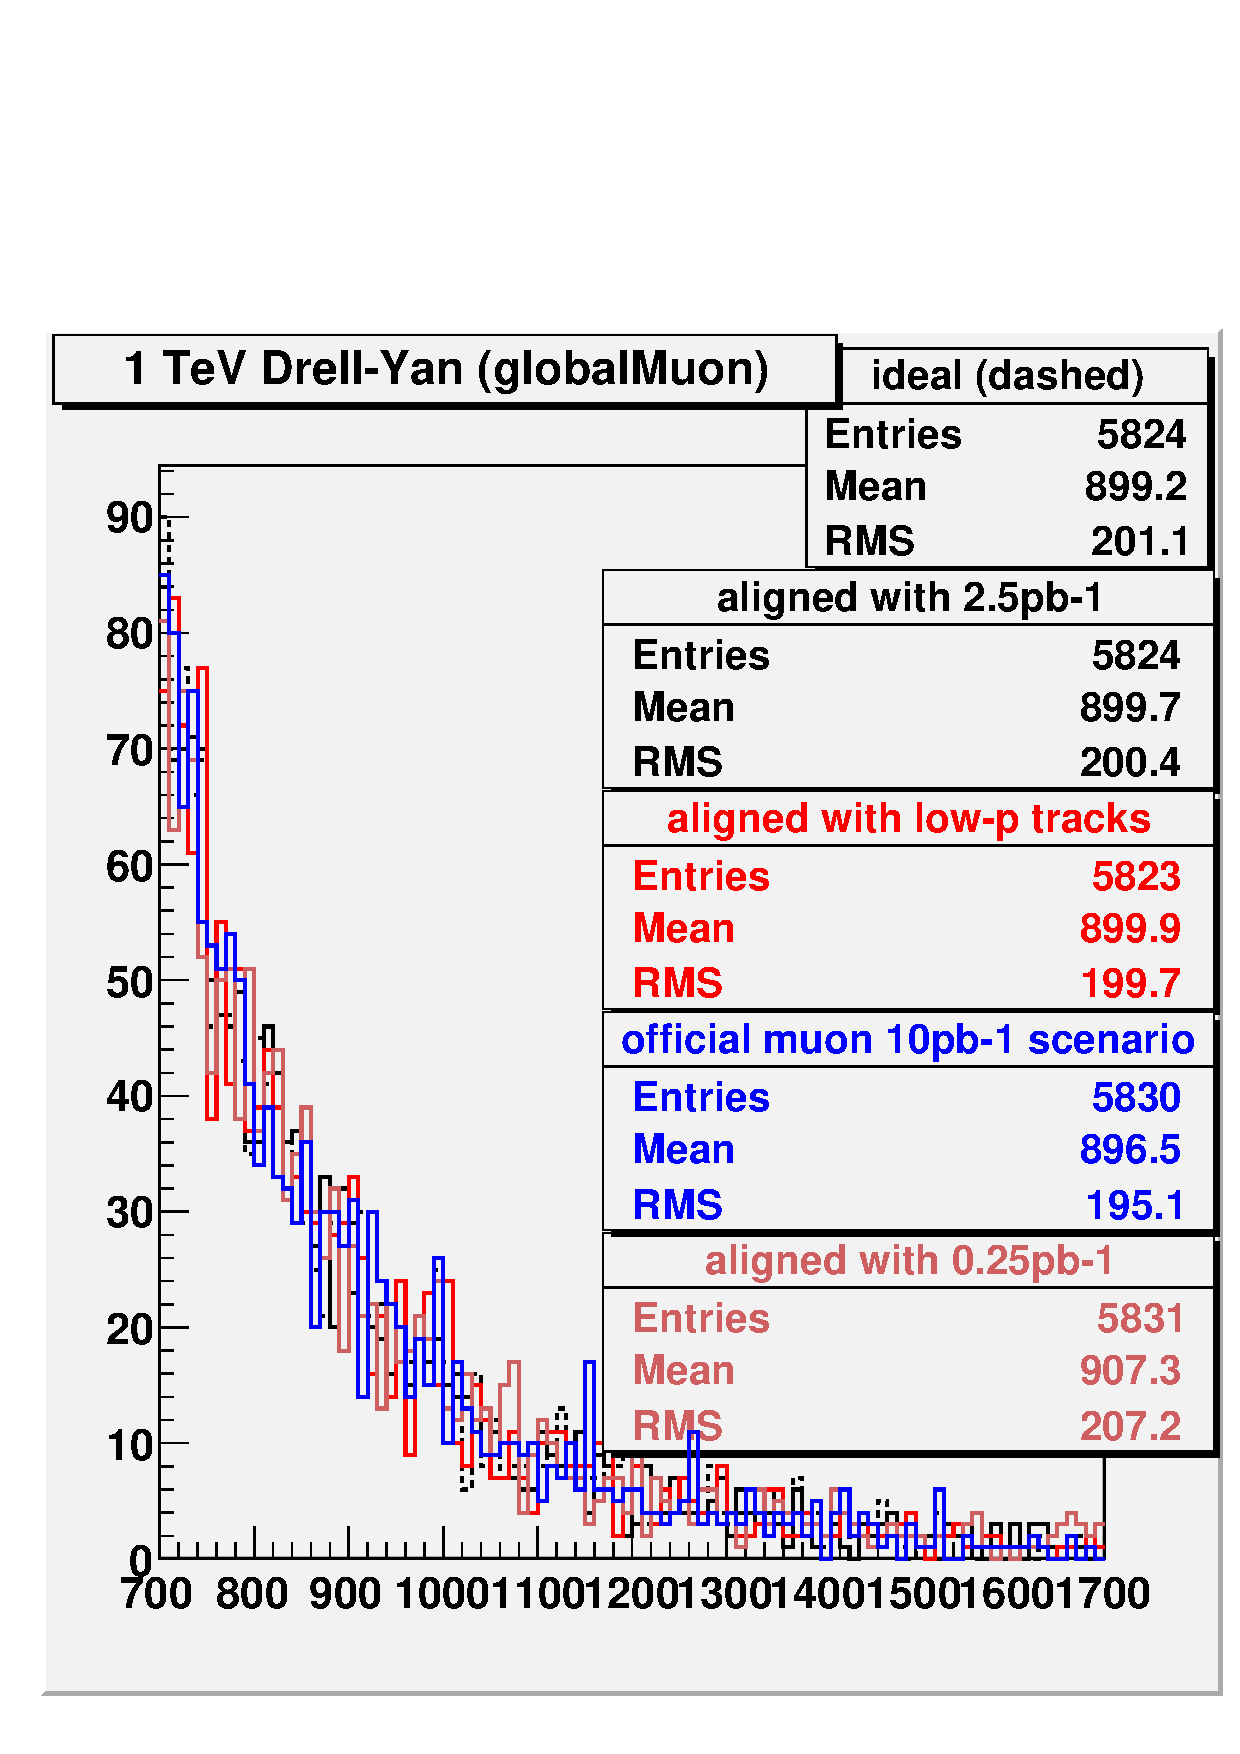
\includegraphics[width=\linewidth]{muoncompare_dy_500.pdf}}
\only<2>{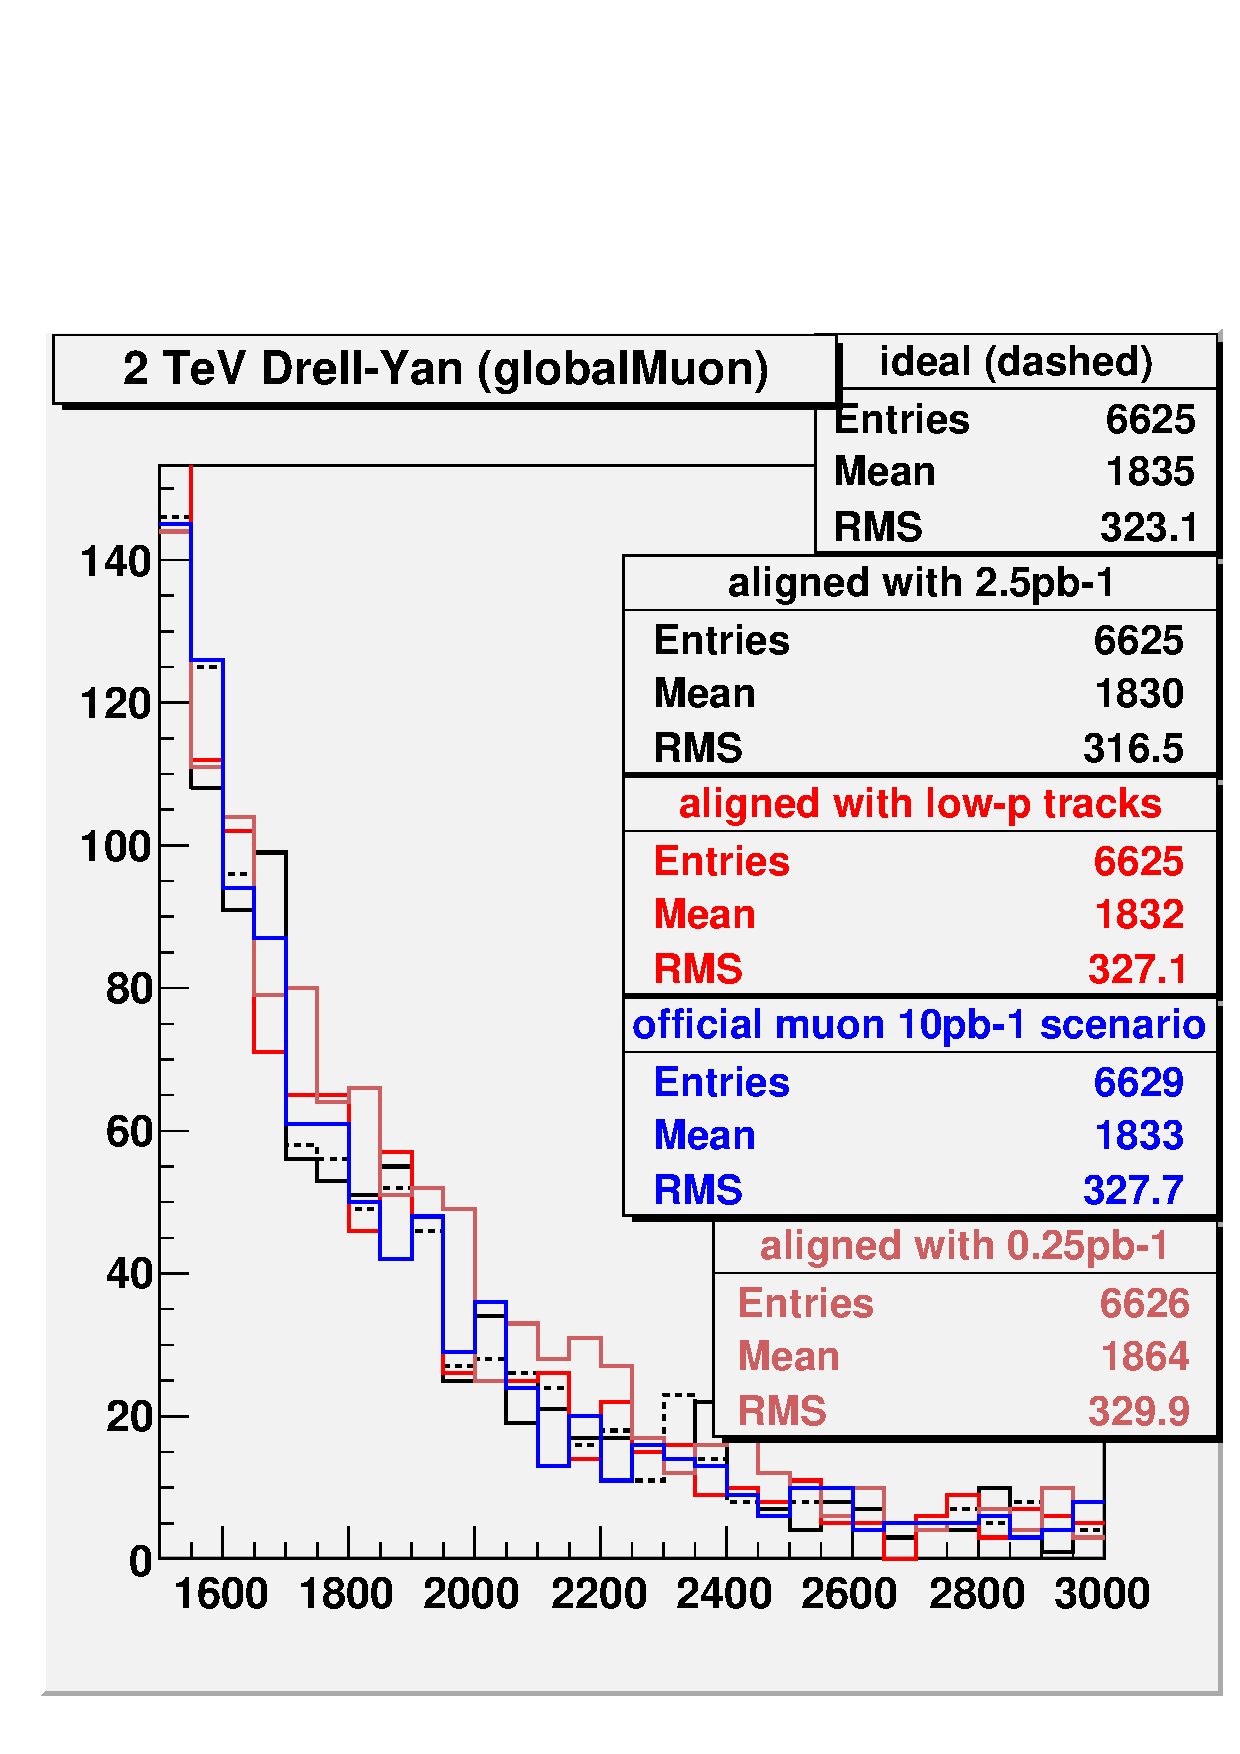
\includegraphics[width=\linewidth]{muoncompare_dy_1000.pdf}}
\column{0.5\linewidth}
\only<1>{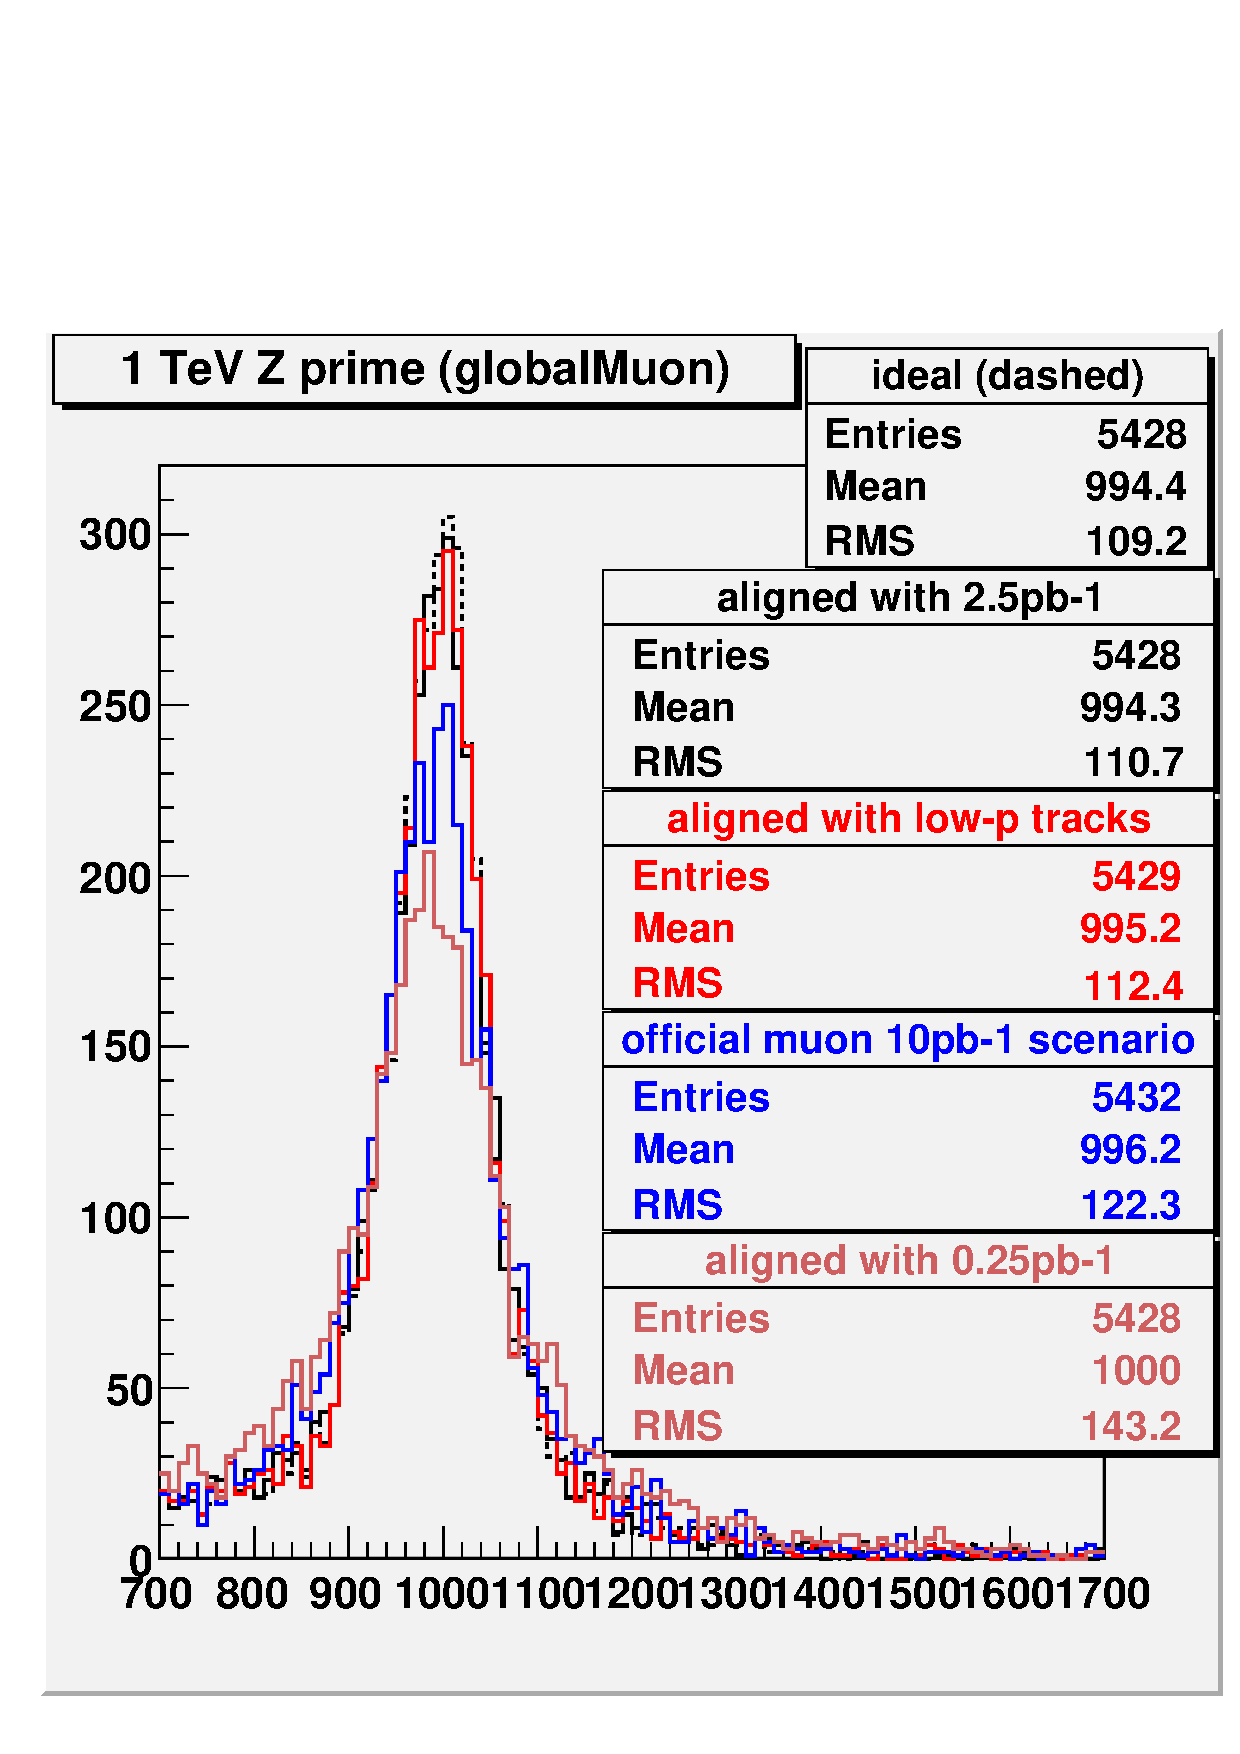
\includegraphics[width=\linewidth]{muoncompare_zprime_1000.pdf}}
\only<2>{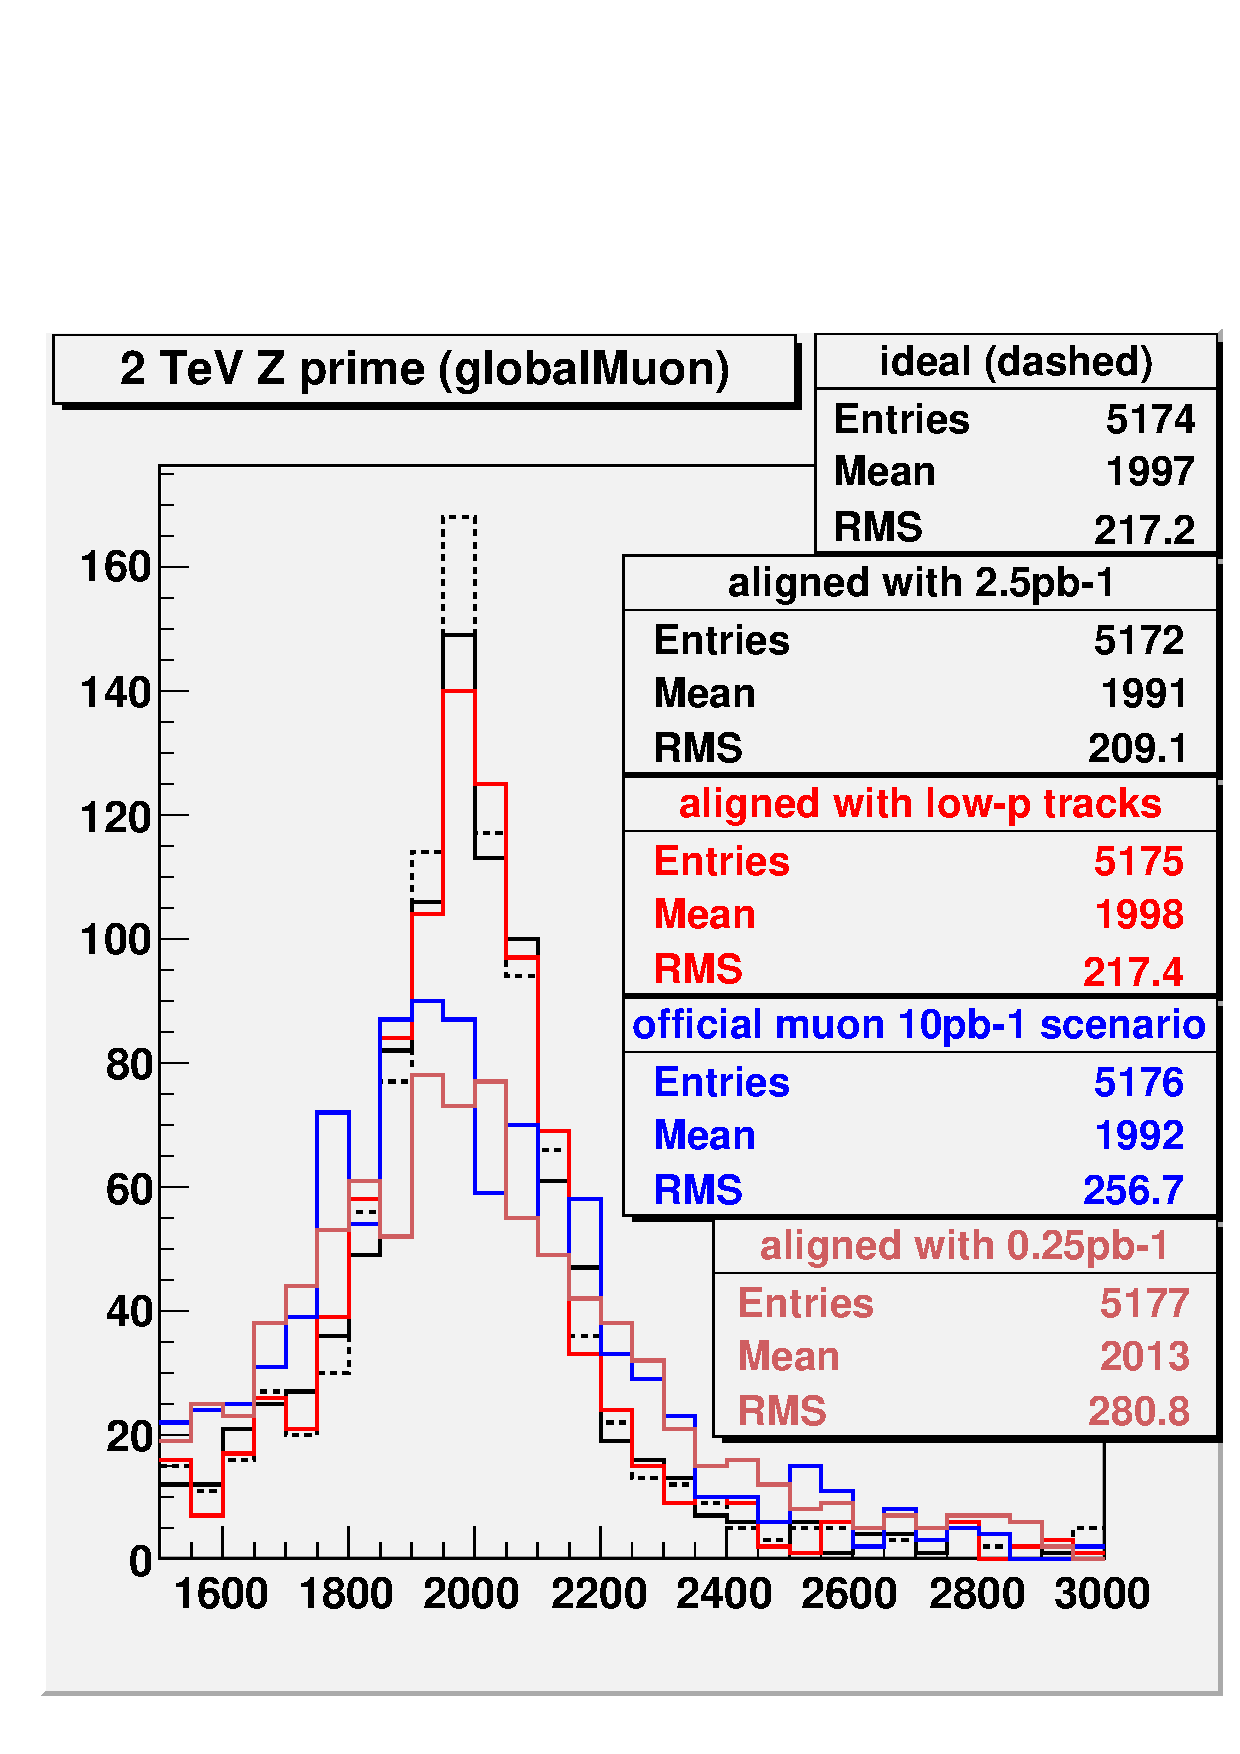
\includegraphics[width=\linewidth]{muoncompare_zprime_2000.pdf}}
\end{columns}

\vspace{0.25 cm}
\textcolor{red}{``low-p'' means 20-60~GeV $Z\to\mu\mu$} \hfill (private 1\_5\_4 $Z'$ samples)

\textcolor{blue}{official 10~pb$^{-1}$ scenario is pessimistic}
\end{frame}

\begin{frame}
\frametitle{Using effect on TeV muons as ``alignment quality''}
\begin{center}
RMS of event-by-event $\displaystyle \frac{\mbox{misaligned di-muon mass}}{\mbox{ideal di-muon mass}} - 1$
\end{center}

\renewcommand{\arraystretch}{1.2}
\begin{tabular}{c c c c c}
Source of alignment & $Z'$(1000) & $Z'$(2000) & \hspace{-0.1cm}DY($>$500)\hspace{-0.1cm} & \hspace{-0.1cm}DY($>$1000)\hspace{-0.1cm} \\\hline
1k $\mu$ (0.25~pb$^{-1}$) & 6.0\% & 5.5\% & 4.8\% & 6.6\% \\
10k $\mu$ (2.5~pb$^{-1}$) & 1.8\% & 1.7\% & 1.6\% & 2.1\% \\
100k $\mu$ (25~pb$^{-1}$) & 1.2\% & 1.1\% & 1.0\% & 1.3\% \\
325k $\mu$ (82~pb$^{-1}$) & 1.0\% & 1.0\% & 0.7\% & 1.2\% \\\hline
$|\vec{p}|$ $>$ 60~GeV & 1.0\% & 1.0\% & 0.8\% & 1.2\% \\
20 $<$ $|\vec{p}|$ $<$ 60~GeV & 1.7\% & 1.7\% & 1.5\% & 2.1\%
\end{tabular}

\vfill\vfill With this as a bottom line, we can make statements like
``switching to $|\vec{p}|$ $>$ 60~GeV is as good as getting a factor of
ten more tracks.''
\end{frame}

\begin{frame}
\frametitle{Uncertainty in track $p_T$, binned in $p_T$ and factorized}
\begin{columns}
\column{0.8\linewidth}
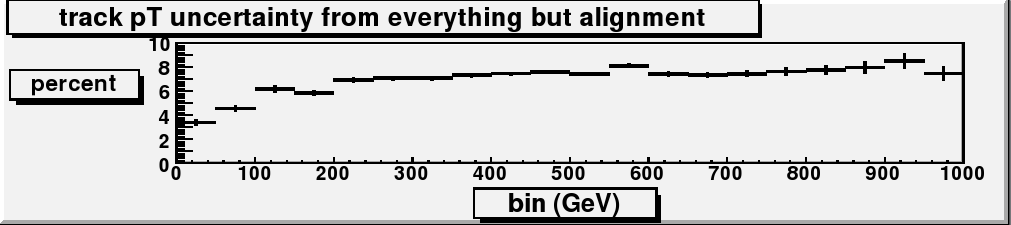
\includegraphics[width=\linewidth]{track_uncertainty_from_all_but_alignment.png}

\only<1>{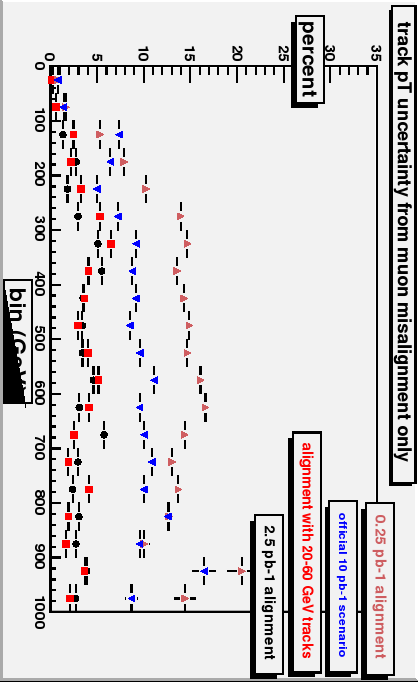
\includegraphics[height=\linewidth, angle=90]{track_uncertainty_from_muon_misalignment.png}}
\only<2>{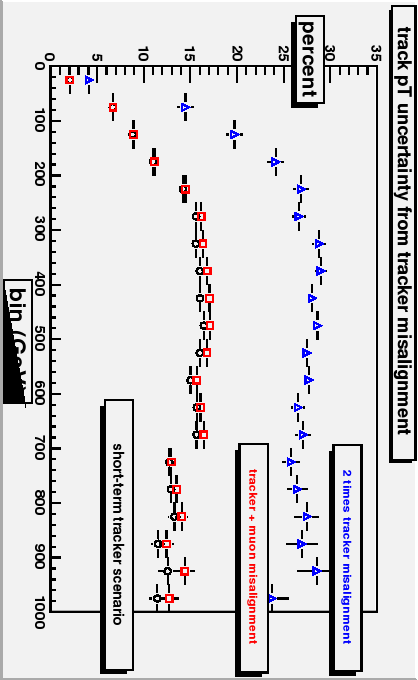
\includegraphics[height=\linewidth, angle=90]{track_uncertainty_from_tracker_misalignment.png}}

\column{0.3\linewidth}
everything but alignment

\vspace{1.5 cm}
effect of alignment

\vspace{1.5 cm}
$\displaystyle \bigg(\frac{\sigma_{p_T}}{p_T}\bigg) = \bigg(\frac{\sigma_\kappa}{\kappa}\bigg)$

\vspace{0.1 cm}
\mbox{$=$ sum in quadrature} \mbox{of both uncertainties}
\end{columns}
\end{frame}

\begin{frame}
\frametitle{Software infrastructure will be tested next Wednesday}
\textcolor{darkblue}{That's when we start our CSA07 jobs}

\begin{center}
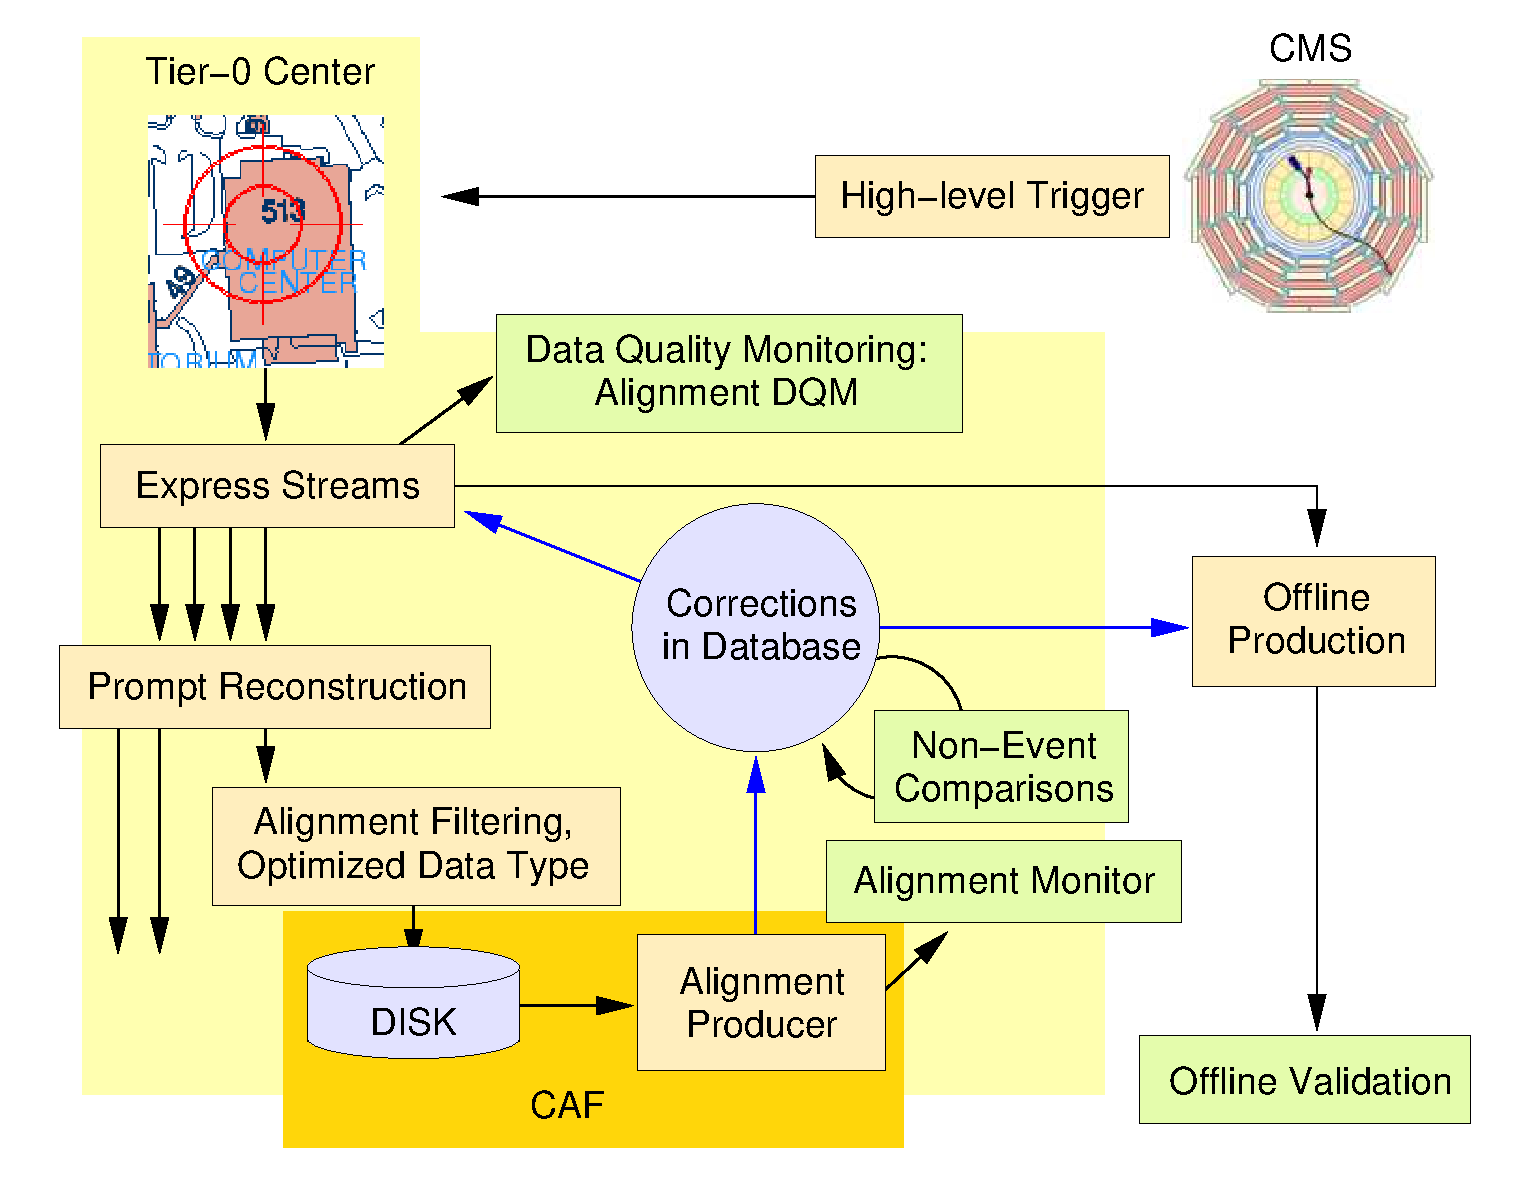
\includegraphics[width=0.75\linewidth]{grand_diagram.pdf}
\end{center}
\end{frame}

\section*{What needs work}

\begin{frame}
\begin{center}
\Huge \textcolor{blue}{\sc Part II: What Needs Work}
\end{center}
\end{frame}

\begin{frame}
\frametitle{ME1/1: bug in alignment and/or reconstruction}
\begin{columns}
\column{0.4\linewidth}
Asymmetric non-Gaussian tail in aligned $y$ positions due to ME1/1
\column{0.6\linewidth}
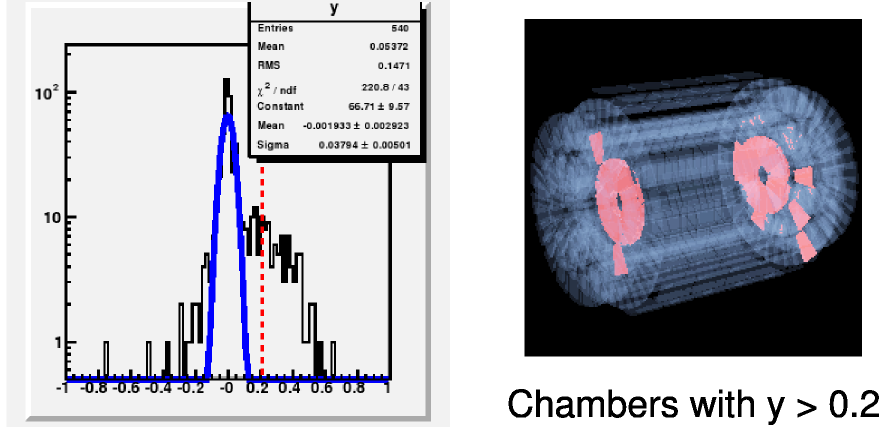
\includegraphics[width=\linewidth]{me11_broken.png}
\end{columns}

\vspace{0.2 cm}
Problem with coordinate systems?  ME1/1's unique geometry?

\vspace{0.2 cm}
Alexey Kamenev (Dubna) and I are beginning investigation\ldots

\vspace{0.2 cm}
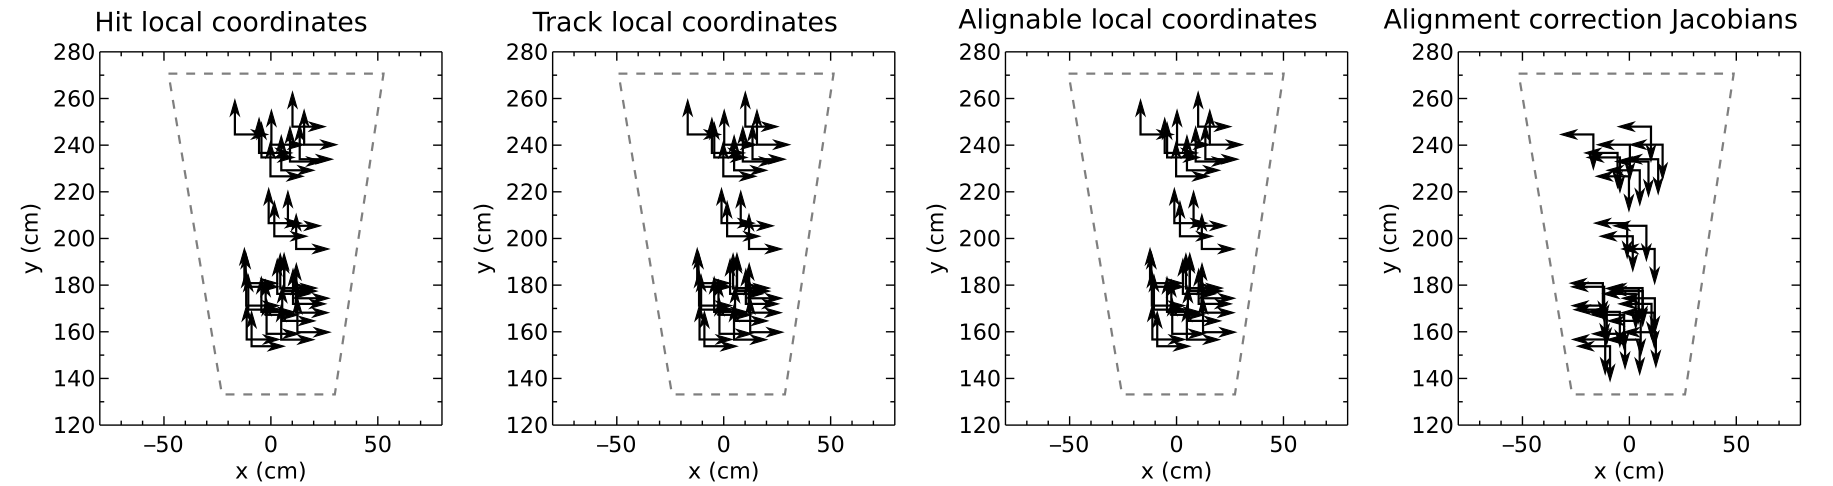
\includegraphics[width=\linewidth]{arrows_side-by-side.png}
\end{frame}

\begin{frame}
\frametitle{Need a more effective procedure for CSC layers}
\begin{itemize}
\item CSC layer misalignment is known (Karoly, Andrey, Oleg\ldots)
\end{itemize}
\begin{center}
\begin{tabular}{c c c}
& current (RMS) & after \textcolor{darkblue}{82~pb$^{-1}$} alignment (RMS) \\\hline
$x$ & 190 $\mu$m & 38 $\mu$m \\
$y$ & 340 $\mu$m & 860 $\mu$m \\
$\phi_z$ & 0.04 mrad & 0.06 mrad \\
\end{tabular}

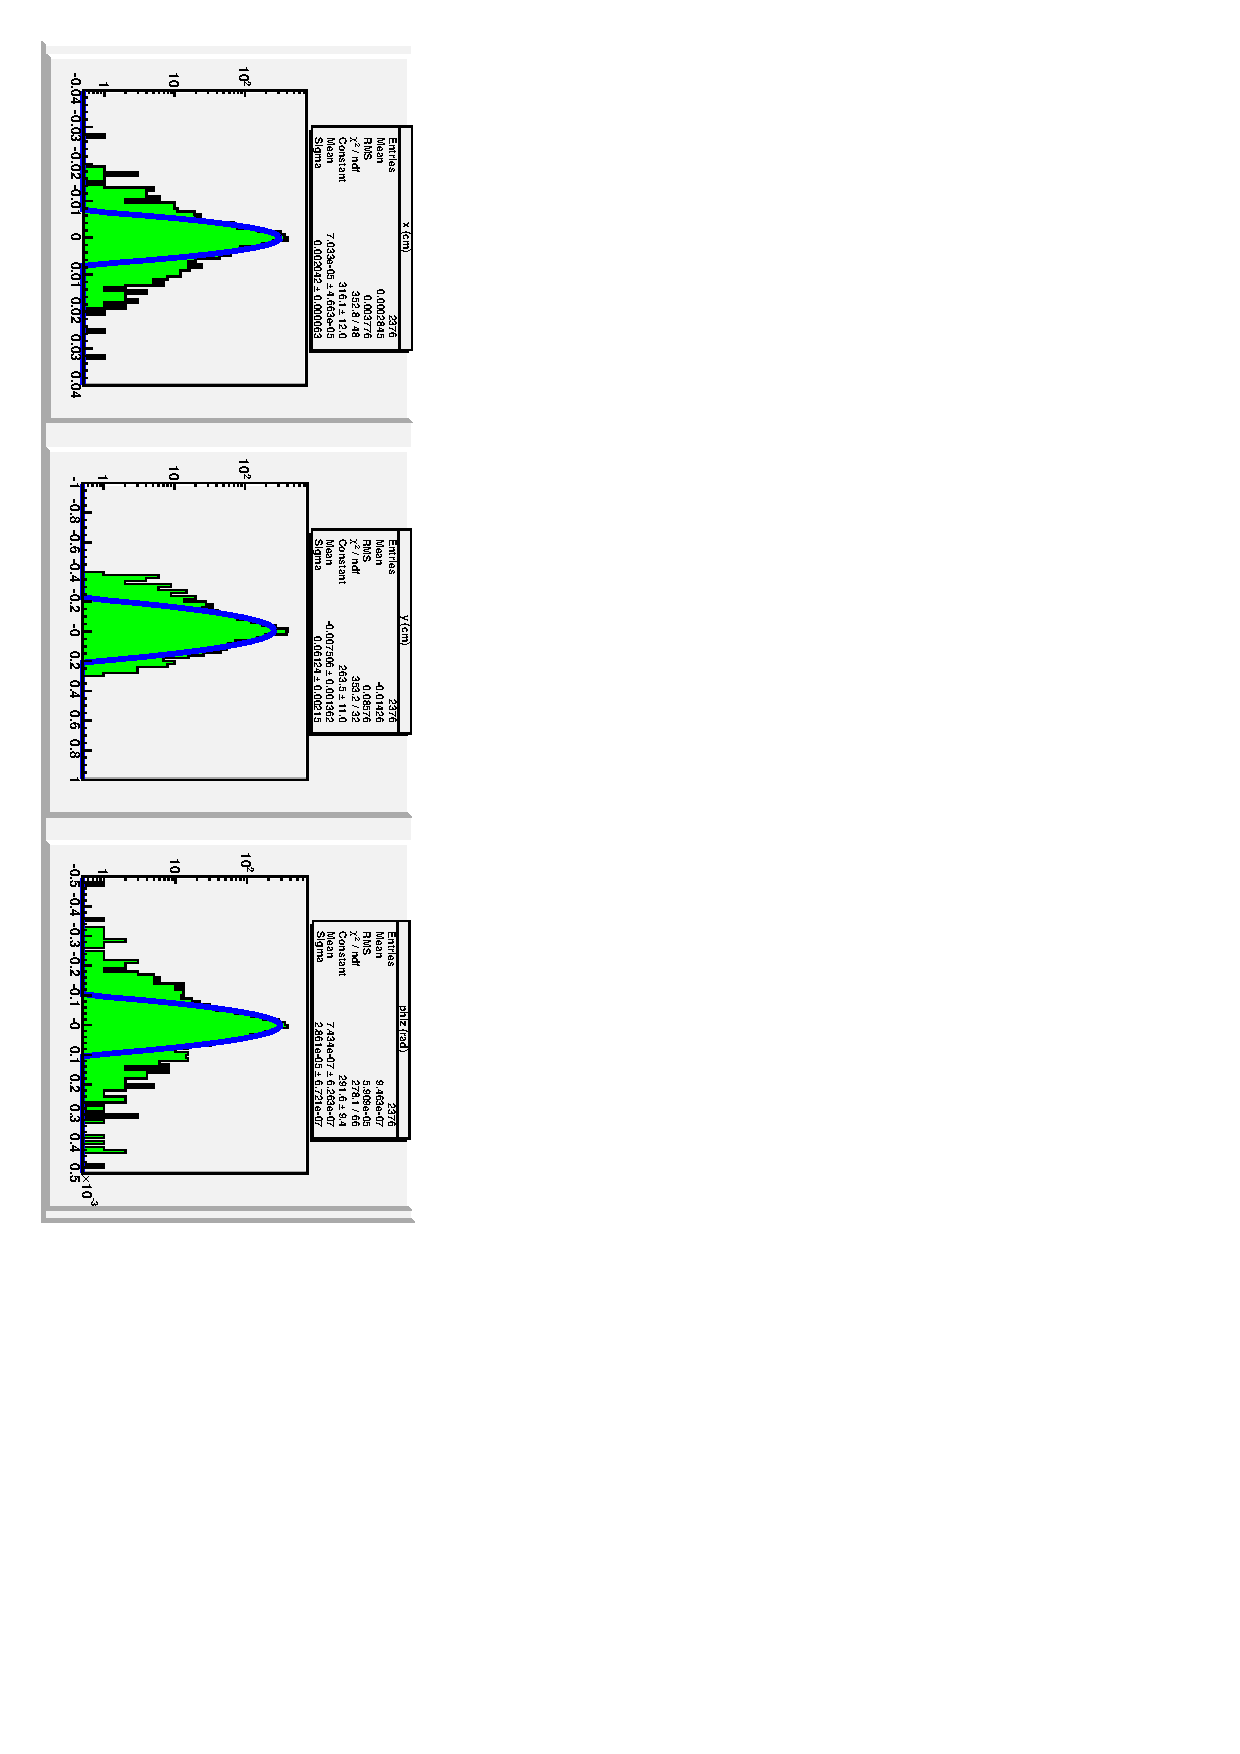
\includegraphics[height=0.9\linewidth, angle=90]{layer_alignment.pdf}
\end{center}

Note: ``alignment quality'' studies use {\it current} layer misalignment
\end{frame}

\section*{Cosmic rays and beam-halo}

\begin{frame}
\begin{center}
\Huge \textcolor{blue}{\sc Part III: Cosmic Rays and Beam-Halo}
\end{center}
\end{frame}

\begin{frame}

{\large \textcolor{darkblue}{Cosmic rays (Alexey Kamenev)}}

\vspace{0.1 cm}
\begin{itemize}\setlength{\itemsep}{0.2 cm}
\item Very recently freed from other obligations, Alexey is ready to work on alignment
\item We're starting with the ME1/1 bug
\item We'll use Adam Roe's re-processed MTCC until official sample becomes available
\end{itemize}

\vfill
{\large \textcolor{darkblue}{Beam-halo (Karoly Banicz)}}

\vspace{0.1 cm}
\begin{itemize}\setlength{\itemsep}{0.2 cm}
\item Generating reliable beam-halo samples
\item Successfully ran an alignment
\item We have yet to optimize the procedure, but the initial results
are promising (I peeked at the output)
\end{itemize}
\end{frame}

\section*{Monitoring tools}

\begin{frame}
\begin{center}
\Huge \textcolor{blue}{\sc Part IV: Tools for Monitoring}
\end{center}
\end{frame}

\begin{frame}

{\large \textcolor{darkblue}{Done}}
\begin{itemize}
\item ``Sanity checks'' generated in the alignment job (used,
for example, to diagnose ME1/1)
\end{itemize}

{\large \textcolor{darkblue}{Started}}
\begin{itemize}
\item Geometry comparison tool: compare alignments at the database level, without events
\end{itemize}

\vspace{0.2 cm}
Example time-series plot: barrel alignments with increasingly misaligned tracker
\begin{center}
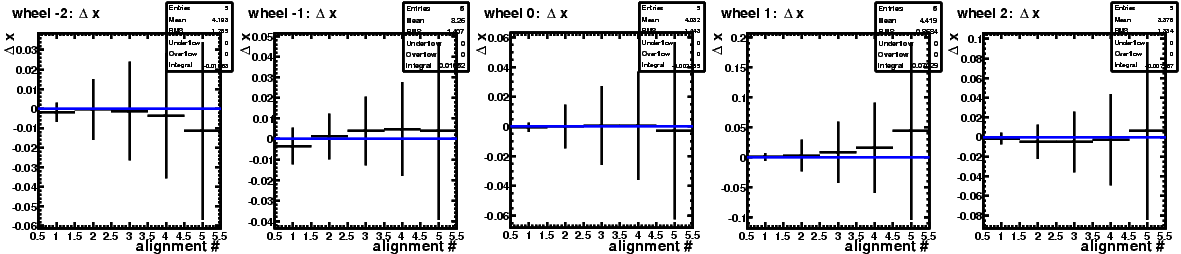
\includegraphics[width=0.9\linewidth]{c_barrel_dxloc.png}
\end{center}

{\large \textcolor{darkblue}{Brand New}}
\begin{itemize}
\item Overlap plots: to identify misaligned chambers {\it in data}\ldots
\end{itemize}
\end{frame}

\begin{frame}
\frametitle{Prerequisites for overlap plots}

\vspace{-0.2 cm}
\begin{center}
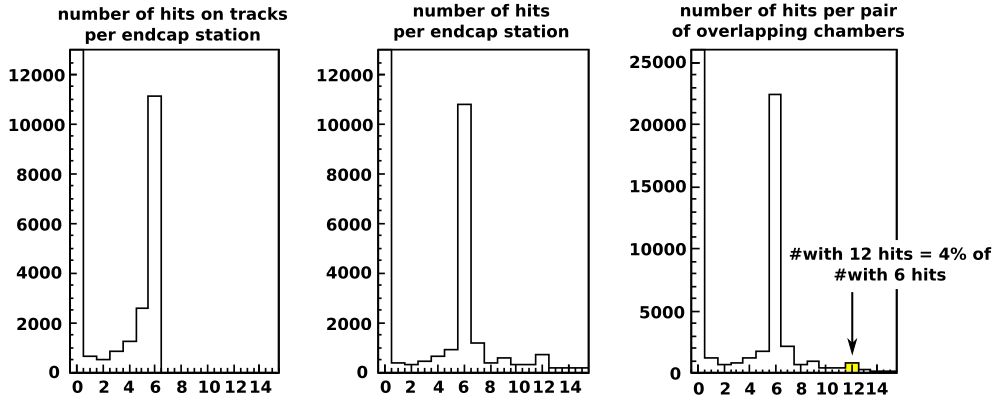
\includegraphics[width=0.85\linewidth]{num_hits.png}
\end{center}

\vspace{-0.2 cm}
\begin{columns}
\column{0.3\linewidth}
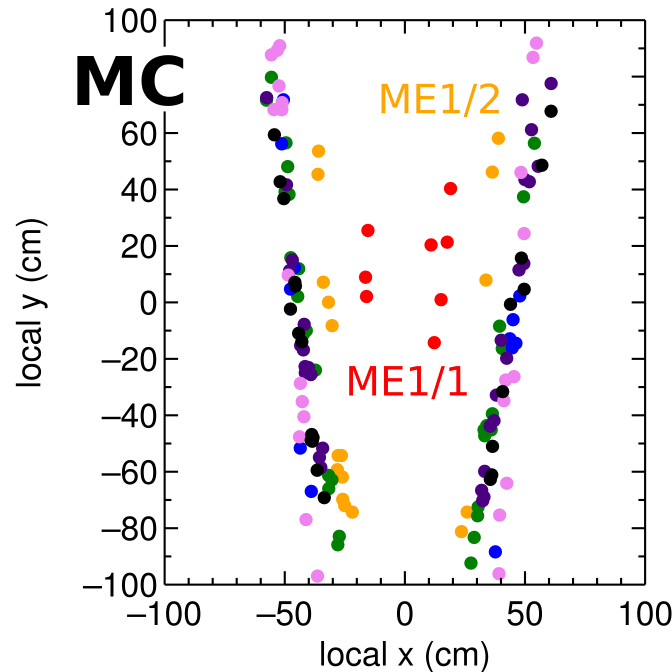
\includegraphics[width=\linewidth]{overlap_positions.png}
\column{0.7\linewidth}
\begin{itemize}
\item No tracks overlap neighboring pairs of chambers in the same station
\item Very few muons do ($\sim$4\%)
\item But 12-hit events usually have segments with good $\chi^2$, in the right regions
\end{itemize}
\end{columns}
\end{frame}

\begin{frame}
\frametitle{Overlap plot (MC)}
\begin{itemize}
\item Linear extrapolation over $\Delta z \approx$ 25~cm
\item Poor resolution, even with all chamber-pairs combined
\item Still have sign ambiguities to resolve
\end{itemize}
\begin{center}
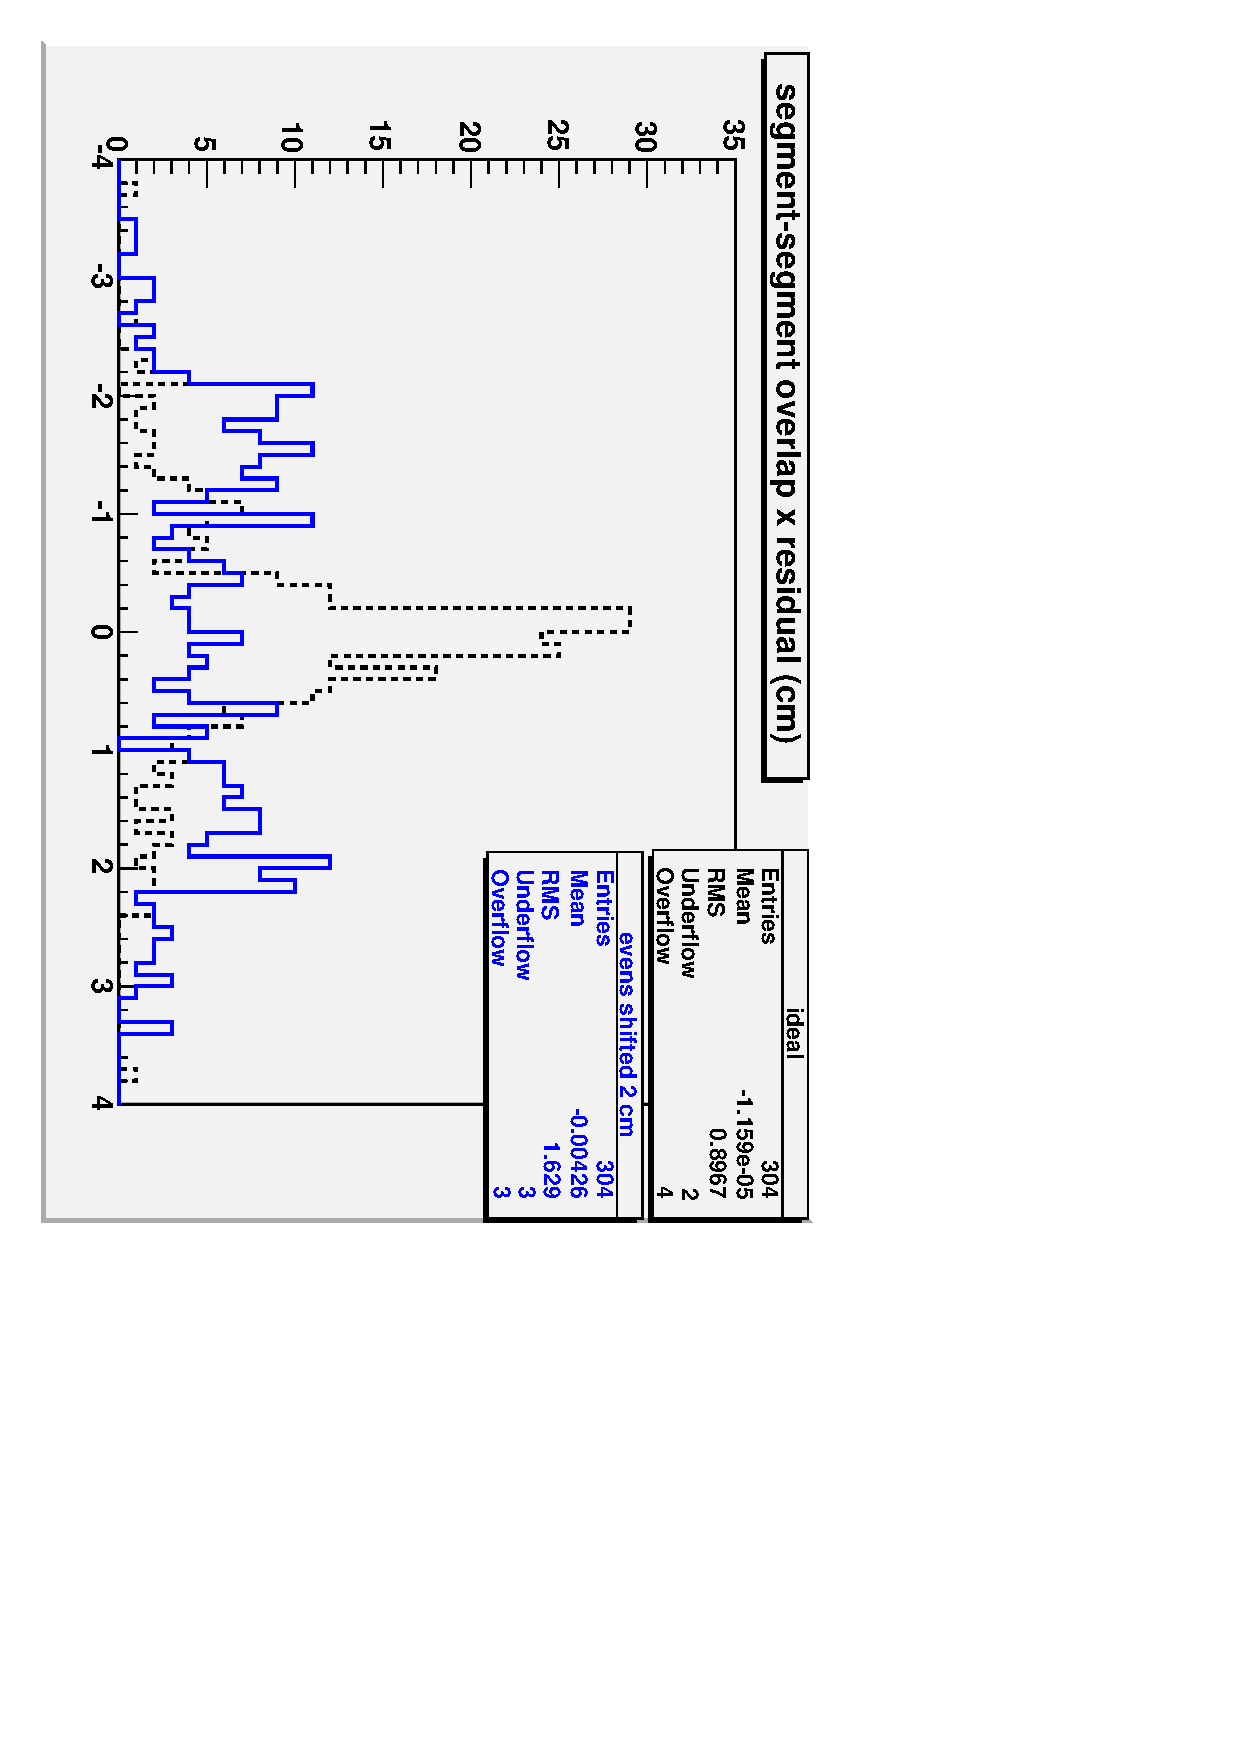
\includegraphics[height=0.8\linewidth, angle=90]{overlap_residual_noMTCC.pdf}
\end{center}
\end{frame}

\section*{Actually aligning the detector}

\begin{frame}
\begin{center}
\Huge \textcolor{blue}{\sc Part V: Toward {\it REAL} Alignments} \\ \textcolor{blue}{(not just realistic)}
\end{center}
\end{frame}

\begin{frame}
\frametitle{Making overlap plots with MTCC}
\begin{tabular}{p{0.32\linewidth} p{0.32\linewidth} p{0.32\linewidth}}
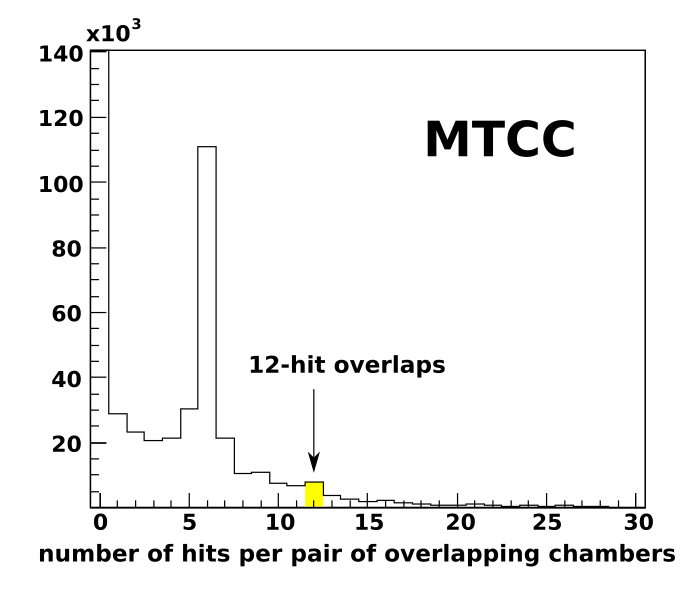
\includegraphics[height=\linewidth]{num_hits_mtcc.png} &
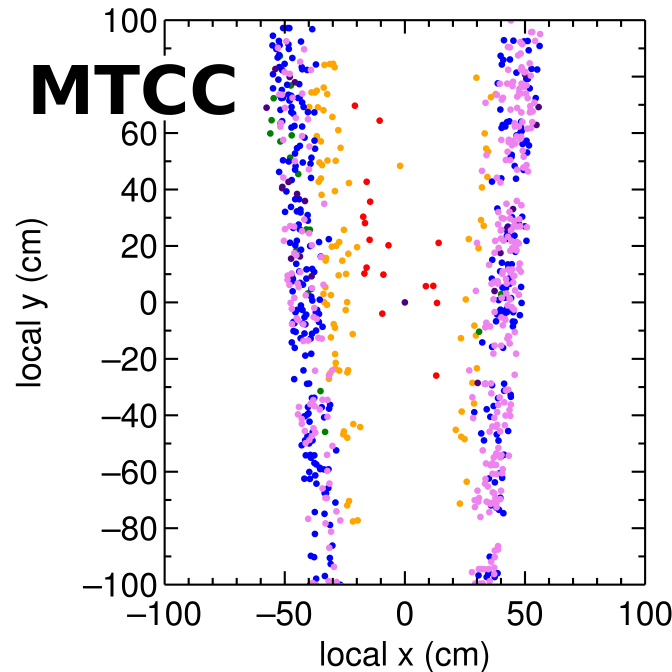
\includegraphics[height=\linewidth]{overlap_positions_mtcc.png} &
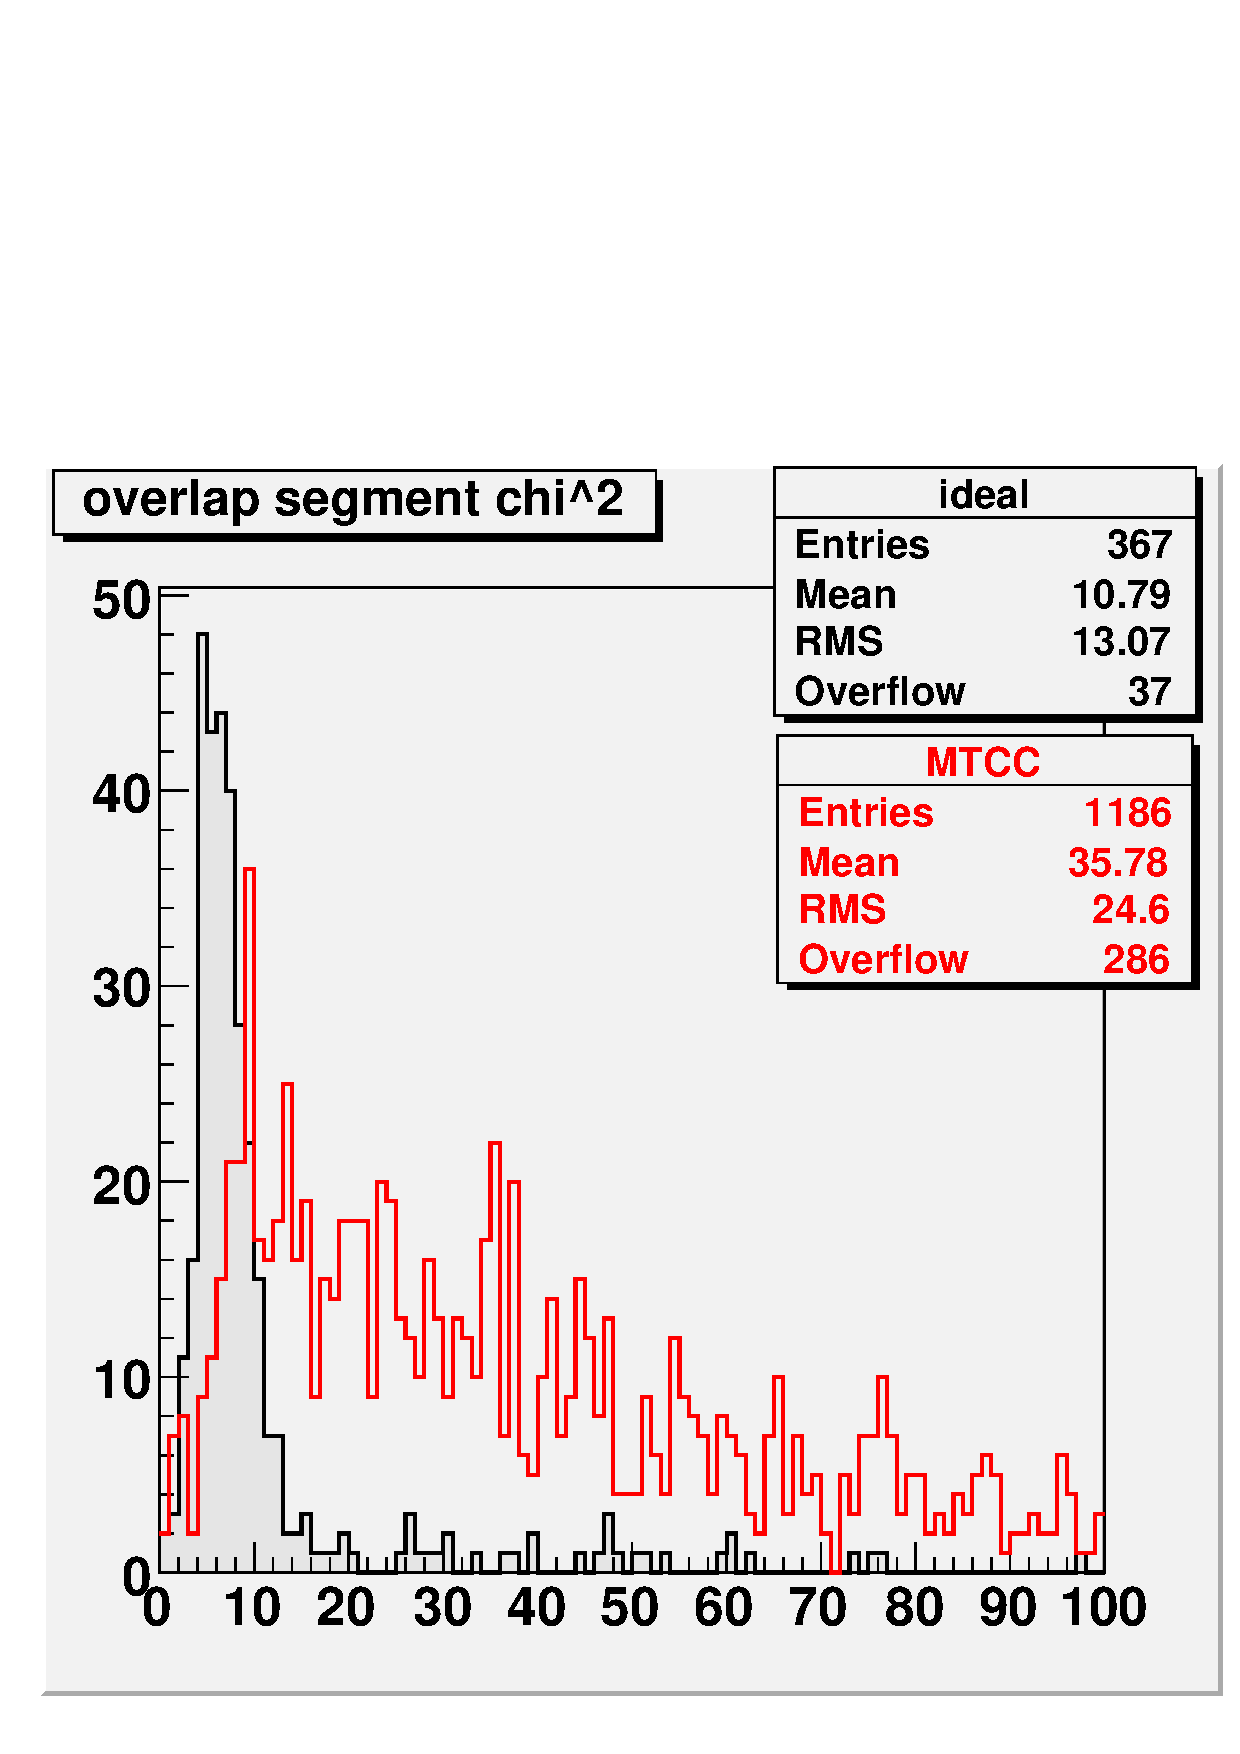
\includegraphics[height=\linewidth]{overlap_chi2.pdf} \\
\end{tabular}

\vfill
\begin{itemize}\setlength{\itemsep}{0.2 cm}
\item Adam Roe's privately re-processed sample
\item Somewhat more background and larger segment $\chi^2$ values
\item Not a fair comparison because:
\begin{itemize}\setlength{\itemsep}{0.1 cm}
\item $Z\to\mu\mu$ MC versus cosmic ray MTCC
\item MTCC layers are misaligned, ideal MC are not
\item MTCC could be miscalibrated, ideal MC is not
\end{itemize}
\end{itemize}
\end{frame}

\begin{frame}
\frametitle{MTCC overlap plot superimposed on MC}
\begin{center}
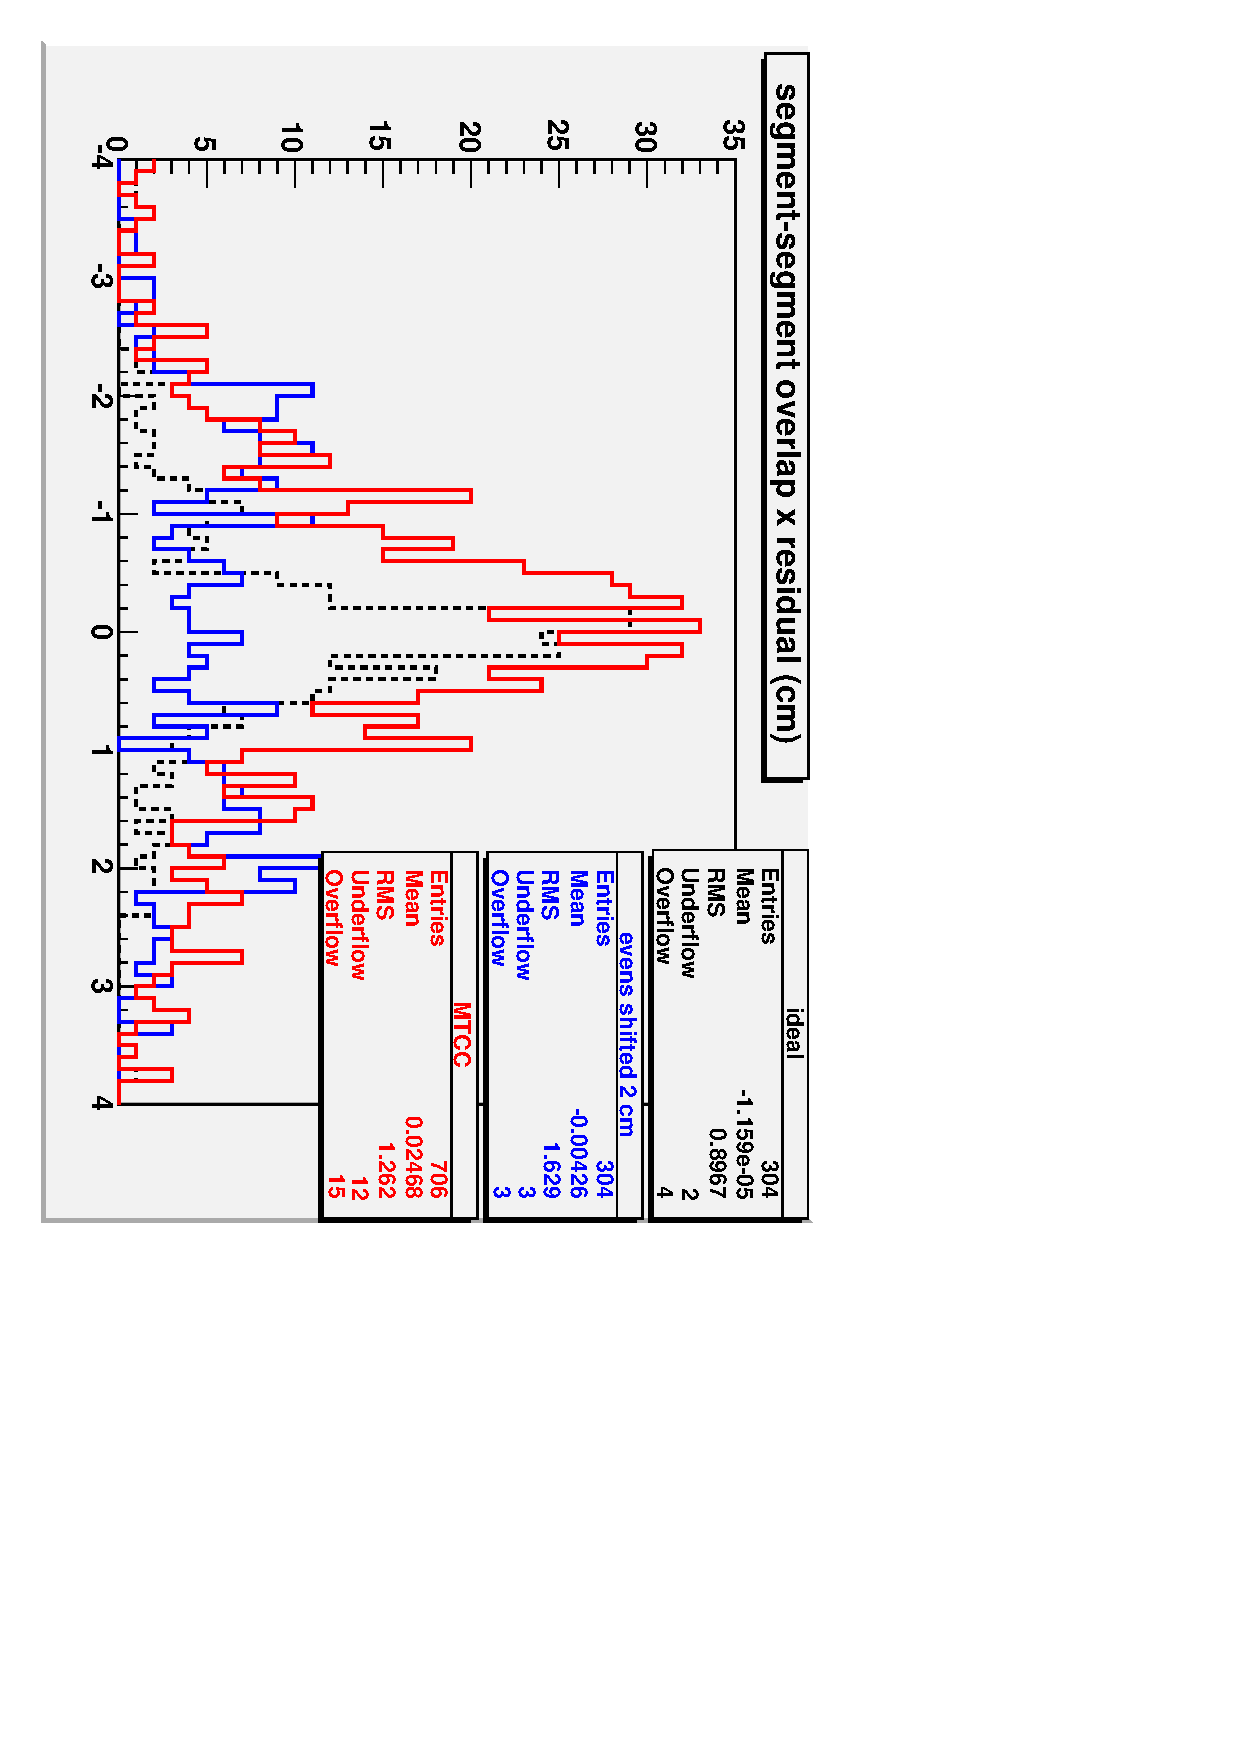
\includegraphics[height=0.8\linewidth, angle=90]{overlap_residual.pdf}
\end{center}
\begin{itemize}
\item Chamber misalignments are probably smaller than $\mathcal{O}(\mbox{1 cm})$
\item How would we see them with 1~cm resolution?
\end{itemize}
\end{frame}

\section*{}

\begin{frame}
\begin{center}
\mbox{ }

\vspace{-1 cm}
\Huge \textcolor{blue}{Conclusions!}
\end{center}
\begin{itemize}\setlength{\itemsep}{0.3 cm}
\item $Z\to\mu\mu$ alignment procedure is not in danger of being late
\item We cautiously anticipate needing only 5~pb$^{-1}$, even with preferring high-$|\vec{p}|$ tracks to high statistics
\item Still checking systematic effects for potential spoilers
\item Still building monitoring tools to catch the problems we don't think of
\item Using TeV muons as a test-bed for alignment quality (in MC)
\item Developing ways to test alignment quality in data
\item MTCC and beam-halo alignment efforts are ramping up
\end{itemize}
\vfill
\mbox{ }
\label{numpages}
\end{frame}

\end{document}
